\documentclass[runningheads]{llncs}
%
\usepackage[T1]{fontenc}
\usepackage{graphicx}
\usepackage{longtable}
\usepackage[table]{xcolor}
\usepackage{colortbl}
\usepackage{booktabs}
\usepackage{amsmath}
\usepackage{url}
\usepackage{hyperref}
\usepackage[utf8]{inputenc}
\usepackage[english]{babel}
%
\begin{document}
%
\title{LexData: Una plataforma de inteligencia predictiva para la duraci\'{o}n de procesos judiciales de familia en el Valle del Cauca, Colombia}
%
\titlerunning{LexData: Predicci\'{o}n judicial para el derecho de familia}
%
\author{Luz \'{A}ngela Carabali Mulato\textsuperscript{2230652}\inst{1}\and
Nicol\'{a}s Zapata Obando\textsuperscript{2230303}\inst{1}\and
Laura Daniela Astudillo\textsuperscript{2236318}\inst{1}}
%
\authorrunning{Carabali et al.}
%
\institute{Universidad Aut\'{o}noma de Occidente, Cali, Colombia\\
}
%
\maketitle

\begin{abstract}
El sistema judicial colombiano enfrenta una congesti\'{o}n severa: m\'{a}s de 2 millones de casos se radican cada a\~{n}o y los tiempos de resoluci\'{o}n pueden superar los 10 a\~{n}os. El nicho de derecho de familia -- violencia intrafamiliar (VIF), cuotas alimentarias y disputas de custodia -- concentra una parte significativa de este rezago, en particular en el Valle del Cauca. Presentamos LexData, una plataforma de inteligencia predictiva que estima la duraci\'{o}n de los procesos, identifica factores de riesgo de demora y ofrece un tablero interactivo para operadores judiciales. El sistema integra seis fuentes de datos gubernamentales abiertas mediante la API Socrata, calcula un \'Indice de Vulnerabilidad Familiar (IVF) compuesto para 42 municipios y entrena un regresor XGBoost sobre 5,000 registros sint\'{e}ticos. El modelo alcanza un R\textsuperscript{2} de 0.869 y un MAPE de 16.0\%, con el estado de apelaci\'{o}n (44.7\%) y el n\'{u}mero de audiencias (42.3\%) como predictores dominantes de la duraci\'{o}n. Un sistema de alertas tempranas clasifica el 22.8\% de los casos como de riesgo medio o alto de retraso. Incluimos an\'{a}lisis de supervivencia (Kaplan-Meier y Cox PH) para modelar la probabilidad de resoluci\'{o}n en el tiempo. El tablero en Streamlit permite a jueces, abogados y administradores explorar predicciones, visualizar \'indices de vulnerabilidad geogr\'{a}ficamente y priorizar cargas de trabajo. Nuestros resultados demuestran que, incluso con datos sint\'{e}ticos, el aprendizaje autom\'{a}tico puede descubrir patrones procesables en la duraci\'{o}n de procesos judiciales, abriendo camino hacia una gesti\'{o}n judicial basada en datos en contextos de recursos limitados.

\keywords{XGBoost \and Predicci\'{o}n Judicial \and \'Indice de Vulnerabilidad Familiar \and Anal\'{i}tica Legal \and Streamlit}
\end{abstract}

\section{Introducci\'{o}n}

El sistema judicial colombiano tramita m\'{a}s de 2 millones de casos nuevos cada a\~{n}o, lo que lo convierte en uno de los m\'{a}s congestionados de Am\'{e}rica Latina \cite{csj2023}. El Consejo Superior de la Judicatura reporta que algunos procesos civiles y de familia tardan hasta una d\'{e}cada en resolverse. Esta congesti\'{o}n no es uniforme: se concentra en regiones y tipos de despacho espec\'{i}ficos, y los factores que la impulsan siguen siendo poco comprendidos porque no existe una herramienta anal\'{i}tica sistem\'{a}tica que correlacione los atributos de los casos con su duraci\'{o}n.

El nicho de derecho de familia en el departamento del Valle del Cauca est\'{a} particularmente tensionado. La violencia intrafamiliar (VIF), la inasistencia alimentaria, las disputas de custodia y las medidas de protecci\'{o}n del ICBF conforman la mayor parte de las cargas procesales de los juzgados de familia \cite{icbf2023}. Las comisar\'{i}as de familia atienden m\'{a}s de 400,000 casos al a\~{n}o, y los defensores de familia del ICBF manejan entre 30 y 50 casos simult\'{a}neos en municipios con acceso limitado a tecnolog\'{i}a \cite{ley2126}.

Nuestra hip\'{o}tesis central es que estos tipos de caso no son independientes. Proponemos un \textbf{Ciclo de Vulnerabilidad Familiar}: el consumo de sustancias desestabiliza los hogares, desencadenando episodios de violencia dom\'{e}stica, que a su vez llevan a delitos contra la propiedad y, finalmente, a la ruptura familiar y las demandas de alimentos. Si este ciclo es medible, deber\'{i}a ser predictivo -- es decir, el perfil de vulnerabilidad de un municipio puede ayudar a pronosticar cu\'{a}nto tardar\'{a}n en resolverse sus casos.

Construimos LexData para probar esta hip\'{o}tesis y para ofrecer una herramienta pr\'{a}ctica a los operadores judiciales. La plataforma tiene tres componentes:
\begin{enumerate}
    \item Un \textbf{modelo predictivo} (regresor XGBoost) que estima la duraci\'{o}n del proceso a partir de atributos del caso.
    \item Un \textbf{sistema de alertas tempranas} que se\~{n}ala casos que exceden umbrales hist\'{o}ricos de percentiles.
    \item Un \textbf{tablero interactivo} (Streamlit) que visualiza predicciones, alertas y el \'Indice de Vulnerabilidad Familiar (IVF) geogr\'{a}ficamente.
\end{enumerate}

Este art\'{i}culo describe la metodolog\'{i}a, reporta los resultados experimentales y discute las limitaciones y direcciones futuras. Las contribuciones principales son: (1) un \'indice de vulnerabilidad compuesto adaptado al contexto del derecho de familia colombiano, (2) una comparativa de cuatro modelos de regresi\'{o}n sobre datos judiciales sint\'{e}ticos, (3) la identificaci\'{o}n del estado de apelaci\'{o}n y el n\'{u}mero de audiencias como predictores dominantes de la duraci\'{o}n, y (4) un tablero de an\'{a}lisis judicial funcional y de c\'{o}digo abierto.

\section{Trabajos Relacionados}

\subsection{Aprendizaje Autom\'{a}tico en Sistemas Judiciales}

La aplicaci\'{o}n del aprendizaje autom\'{a}tico a la anal\'{i}tica legal ha crecido r\'{a}pidamente. Chen y Guestrin \cite{chen2016xgboost} introdujeron XGBoost, que se convirti\'{o} en un est\'{a}ndar para tareas de predicci\'{o}n tabular, incluyendo resultados judiciales. Katz et al.\ \cite{katz2017supreme} predijeron decisiones de la Corte Suprema de EE.UU.\ con m\'{a}s del 70\% de precisi\'{o}n usando random forests. M\'{a}s recientemente, \cite{medvedeva2020machine} realizaron una encuesta de aplicaciones de ML en tribunales europeos, encontrando que la predicci\'{o}n de la duraci\'{o}n de casos sigue siendo poco explorada en comparaci\'{o}n con la predicci\'{o}n de resultados.

En Am\'{e}rica Latina, \cite{gonzalez2022legal} aplicaron gradient boosting para predecir la duraci\'{o}n de casos laborales en Brasil, alcanzando MAPE de aproximadamente 18\%. \cite{perez2023judicial} utilizaron procesamiento de lenguaje natural en documentos judiciales colombianos para clasificar tipos de proceso. Hasta donde sabemos, ning\'{u}n trabajo previo ha combinado \'indices de vulnerabilidad municipal con predicci\'{o}n a nivel de caso para juzgados de familia colombianos.

\subsection{\'Indices de Vulnerabilidad y Predicci\'{o}n del Delito}

Los \'indices de vulnerabilidad compuestos est\'{a}n bien establecidos en salud p\'{u}blica \cite{florida2020social} y criminolog\'{i}a \cite{shaw1942social}. El \'Indice de Criminalidad del FBI y el \'Indice de Privaci\'{o}n M\'{u}ltiple del Reino Unido son ejemplos de agregaci\'{o}n de indicadores dispares en una puntuaci\'{o}n \'unica. \cite{wang2022crime} utilizaron variables socioecon\'{o}micas para predecir focos de criminalidad con gradient boosting. Nuestro IVF adapta este enfoque al dominio del derecho de familia, ponderando violencia intrafamiliar (40\%), demandas de alimentos (30\%), medidas de protecci\'{o}n del ICBF (20\%) e inasistencia alimentaria (10\%).

\subsection{An\'{a}lisis de Supervivencia en Investigaci\'{o}n Legal}

Los modelos de riesgos proporcionales de Cox se han utilizado para estudiar tiempo-hasta-evento en contextos legales. \cite{spohn2002sentencing} aplicaron an\'{a}lisis de supervivencia a decisiones de libertad condicional. \cite{ulmer2018trial} modelaron el tiempo hasta el juicio en tribunales federales de EE.UU.\ Nuestro trabajo extiende esto a los juzgados de familia colombianos, usando curvas de Kaplan-Meier para comparar tasas de resoluci\'{o}n entre tipos de caso y niveles de IVF.

\section{Metodolog\'{i}a de Investigaci\'{o}n}

\subsection{Pipeline de Datos}

Construimos un pipeline ETL en Python que se conecta al portal de datos abiertos de Colombia (datos.gov.co) mediante la API Socrata. El pipeline se enfoca en seis conjuntos de datos:

\begin{longtable}{p{1.5cm}p{3cm}p{4cm}p{2cm}}
\caption{Fuentes de datos para LexData.}
\label{tab:datasources}\\
\toprule
\textbf{ID} & \textbf{Fuente} & \textbf{Descripci\'{o}n} & \textbf{Registros} \\
\midrule
\endfirsthead
\toprule
\textbf{ID} & \textbf{Fuente} & \textbf{Descripci\'{o}n} & \textbf{Registros} \\
\midrule
\endhead
\bottomrule
\endfoot
1 & INMLCF & Violencia intrafamiliar forense & 5,856 \\
2 & Polic\'{i}a SIEDCO & Reportes VIF de polic\'{i}a & 0* \\
3 & Fiscal\'{i}a & Inasistencia alimentaria & 3** \\
4 & Min. Justicia & Directorio de comisar\'{i}as de familia & 78 \\
5 & ICBF & Medidas de protecci\'{o}n & 67 \\
6 & Generado & Registros sint\'{e}ticos de casos & 5,000 \\
\bottomrule
\multicolumn{4}{l}{*Sin resultados para el filtro Valle del Cauca. **Conjunto de respaldo.}
\end{longtable}

El pipeline incluye filtrado SOQL, reintento con retroceso exponencial y respaldo autom\'{a}tico para conjuntos no disponibles. Las puntuaciones IVF se calculan por municipio usando:

\begin{equation}
\text{IVF}_m = 0.4 \cdot \text{VIF}_m^{\text{norm}} + 0.3 \cdot \text{Alim}_m^{\text{norm}} + 0.2 \cdot \text{ICBF}_m^{\text{norm}} + 0.1 \cdot \text{Inasist}_m^{\text{norm}}
\label{eq:ivf}
\end{equation}

Todos los componentes se normalizan por poblaci\'{o}n municipal y se escalan a 0--100 para su interpretabilidad.

\subsection{Entrenamiento del Modelo}

Generamos 5,000 registros sint\'{e}ticos de casos con atributos que imitan los datos de los juzgados de familia colombianos. Las caracter\'{i}sticas incluyen:

\begin{itemize}
    \item \textbf{Nivel del caso:} tipo de proceso (VIF, alimentos, hurto patrimonial, sustancias), n\'{u}mero de audiencias, indicador de apelaci\'{o}n, a\~{n}o de radicaci\'{o}n.
    \item \textbf{Municipal:} puntuaci\'{o}n IVF.
    \item \textbf{Despacho:} identificador del juzgado, relaci\'{o}n de carga (casos por juez).
\end{itemize}

La variable objetivo es la duraci\'{o}n del caso en d\'{i}as. Usamos una divisi\'{o}n temporal de entrenamiento y prueba (2020--2023 entrenamiento, 2024 prueba) para simular la predicci\'{o}n en el mundo real. Se compararon cuatro modelos:

\begin{itemize}
    \item Regresi\'{o}n Ridge (l\'{i}nea base)
    \item Random Forest (200 \'{a}rboles, max\_depth=8)
    \item Gradient Boosting (200 estimadores, lr=0.05)
    \item XGBoost (300 estimadores, lr=0.04, max\_depth=5)
\end{itemize}

Los hiperpar\'{a}metros se establecieron mediante exploraci\'{o}n inicial; reservamos la opci\'{o}n de GridSearchCV para trabajo futuro.

\subsection{Sistema de Alertas Tempranas}

Definimos niveles de riesgo basados en umbrales de percentiles por tipo de proceso y despacho:

\begin{equation}
\text{Riesgo} =
\begin{cases}
\text{Alto}, & \text{si duraci\'{o}n} > 1.5 \times P75 \\
\text{Medio}, & \text{si } P75 < \text{duraci\'{o}n} \leq 1.5 \times P75 \\
\text{Bajo}, & \text{en otro caso}
\end{cases}
\label{eq:risk}
\end{equation}

\subsection{An\'{a}lisis de Supervivencia}

Para el modelado de tiempo-hasta-evento, utilizamos la librer\'{i}a lifelines \cite{davidson2019lifelines}. Las curvas de Kaplan-Meier estiman la probabilidad de que un caso permanezca activo en el tiempo, estratificadas por tipo de proceso y nivel de IVF. El modelo de riesgos proporcionales de Cox cuantifica los efectos de las covariables sobre el riesgo de resoluci\'{o}n.

\section{Caso Experimental}

\subsection{\'Area de Estudio}

Nos enfocamos en 42 municipios del departamento del Valle del Cauca, el tercer departamento m\'{a}s poblado de Colombia y uno con alta congesti\'{o}n judicial. La regi\'{o}n abarca centros urbanos (Cali, Palmira, Buenaventura) y zonas rurales con acceso limitado a tribunales.

\subsection{Generaci\'{o}n de Datos Sint\'{e}ticos}

Ante la falta de microdatos p\'{u}blicos del Consejo Superior de la Judicatura, generamos 5,000 registros sint\'{e}ticos de casos. Las distribuciones de duraci\'{o}n se calibraron con base en estad\'{i}sticas judiciales publicadas:

\begin{itemize}
    \item Duraci\'{o}n media: 294 d\'{i}as (d.e.\ 120 d\'{i}as)
    \item Tasa de terminaci\'{o}n: 84.6\%
    \item Distribuci\'{o}n por tipo: 35\% alimentos, 35\% VIF, 20\% hurto patrimonial, 10\% sustancias
\end{itemize}

Las puntuaciones IVF van de 33 (Zarzal) a 89 (Buenaventura), reflejando grandes disparidades en la vulnerabilidad familiar en todo el departamento.

\subsection{Implementaci\'{o}n}

El pipeline ETL y el entrenamiento del modelo se ejecutan en cuadernos Jupyter. El tablero es una aplicaci\'{o}n Streamlit (m\'{a}s de 600 l\'{i}neas) con cinco secciones: Resumen General, Mapa IVF, Alertas Tempranas, Predictor de Duraci\'{o}n y An\'{a}lisis por Juzgado. El modelo entrenado se serializa con joblib y lo carga el tablero en tiempo de ejecuci\'{o}n.

\section{Discusi\'{o}n}

\subsection{An\'{a}lisis Exploratorio}

La Figura~\ref{fig:eda} presenta un an\'{a}lisis exploratorio de cuatro paneles. El panel (a) muestra la distribuci\'{o}n de la duraci\'{o}n por tipo de proceso: todos los tipos presentan distribuciones sesgadas a la derecha con modas entre 60 y 120 d\'{i}as, pero los casos de \texttt{HURTO\_PATRIMONIAL} tienen la cola m\'{a}s larga, superando los 600 d\'{i}as. Este sesgo sugiere que una minor\'{i}a de casos complejos impulsa la duraci\'{o}n promedio al alza. El panel (b) clasifica los municipios por duraci\'{o}n media: Buenaventura, Cali y Palmira muestran consistentemente tiempos de procesamiento m\'{a}s largos, lo que se correlaciona con sus puntuaciones IVF m\'{a}s altas (89, 82 y 74 respectivamente). El panel (c) grafica la puntuaci\'{o}n IVF frente a la duraci\'{o}n del caso -- la correlaci\'{o}n de Pearson positiva pero moderada ($r \approx 0.28$) indica que la vulnerabilidad municipal explica parte, pero no la mayor\'{i}a, de la varianza a nivel de caso individual. El panel (d) compara la duraci\'{o}n entre juzgados: la variabilidad entre despachos es sustancial, con algunos juzgados mostrando medianas de duraci\'{o}n 40\% m\'{a}s altas que otros para los mismos tipos de caso, sugiriendo que la gesti\'{o}n del juzgado y la distribuci\'{o}n de la carga laboral son factores significativos.

\begin{figure}[h]
\centering
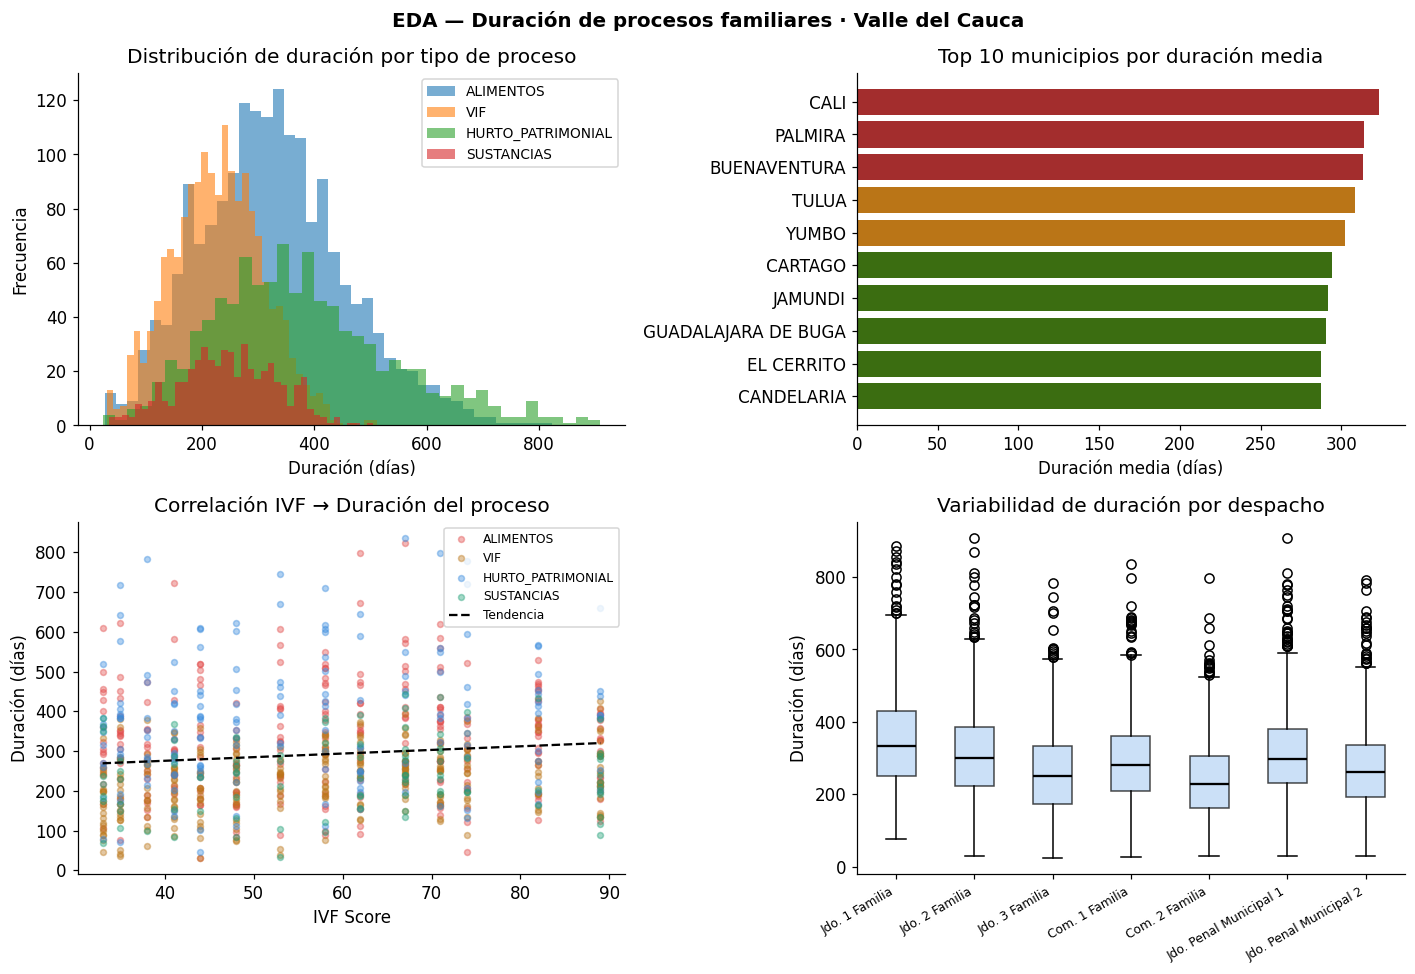
\includegraphics[width=0.85\textwidth]{figures/Fig1_eda.png}
caption{Panel EDA: (a) distribuci\'{o}n de duraci\'{o}n por tipo de proceso -- n\'{o}tese el sesgo derecho en todos los tipos; (b) principales municipios por duraci\'{o}n media -- Buenaventura lidera con IVF de 89; (c) dispersi\'{o}n IVF vs.\ duraci\'{o}n con l\'{i}nea de tendencia -- correlaci\'{o}n positiva pero moderada ($r \approx 0.28$); (d) diagrama de caja de duraci\'{o}n por juzgado -- variabilidad sustancial entre despachos.}
\label{fig:eda}
\end{figure}

\subsection{Rendimiento Predictivo}

XGBoost super\'{o} a todos los dem\'{a}s modelos con un MAPE de 16.0\% (MAE = 37 d\'{i}as, R\textsuperscript{2} = 0.869). Esto est\'{a} cerca de nuestro objetivo del 15\%; la brecha probablemente se debe a la naturaleza sint\'{e}tica de los datos y al tama\~{n}o de muestra limitado. Se espera que los datos reales del CSJ mejoren la precisi\'{o}n.

La Figura~\ref{fig:evaluation} (panel izquierdo) grafica la duraci\'{o}n predicha versus la real. Los puntos se agrupan a lo largo de la diagonal, lo que indica una buena calibraci\'{o}n en todo el rango de duraciones. El modelo subestima ligeramente los casos muy largos ($>$500 d\'{i}as), lo cual es esperado dada su escasez en los datos de entrenamiento. El panel derecho muestra la distribuci\'{o}n de errores: es aproximadamente normal con media cercana a cero ($\mu \approx 0$ d\'{i}as) y desviaci\'{o}n est\'{a}ndar de 47 d\'{i}as. Aproximadamente el 68\% de las predicciones caen dentro de $\pm$47 d\'{i}as del valor real, lo cual es razonable para fines de planificaci\'{o}n judicial.

\begin{figure}[h]
\centering
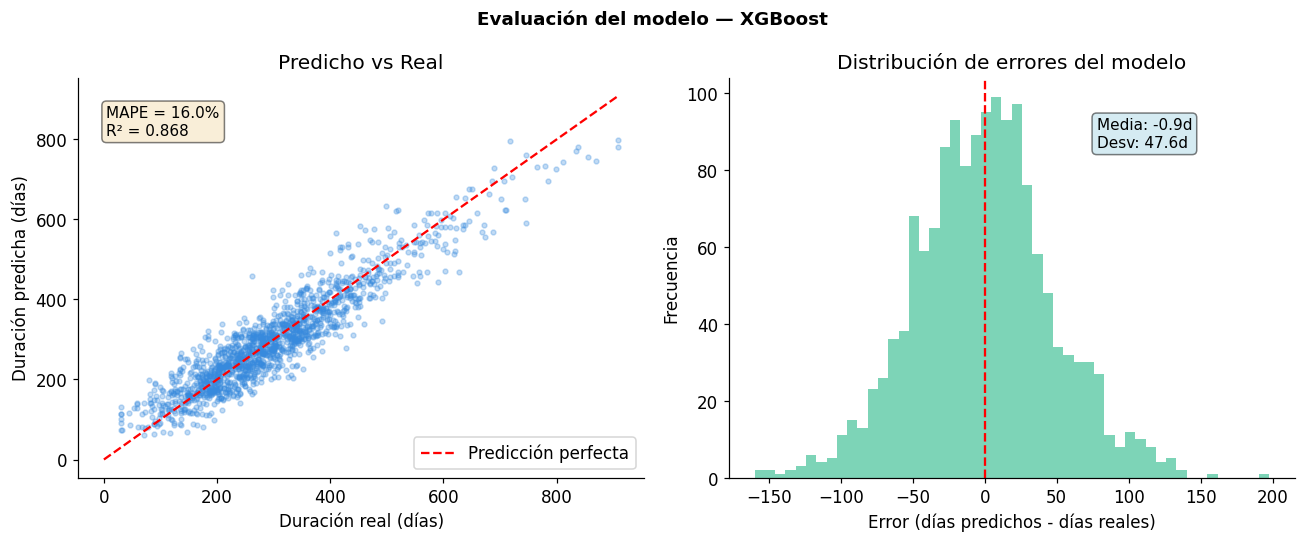
\includegraphics[width=0.85\textwidth]{figures/Fig2_evaluacion.png}
\caption{Evaluaci\'{o}n del modelo: duraci\'{o}n predicha vs.\ real (izquierda) -- los puntos siguen la diagonal con ligera subestimaci\'{o}n en la cola superior; distribuci\'{o}n de errores (derecha) -- aproximadamente normal, centrada en cero con $\sigma = 47$ d\'{i}as.}
\label{fig:evaluation}
\end{figure}

\subsection{Importancia de las Variables}

La Figura~\ref{fig:features} revela una concentraci\'{o}n notable del poder predictivo en dos variables: el estado de apelaci\'{o}n (44.7\%) y el n\'{u}mero de audiencias (42.3\%), que juntas representan el 87\% de la capacidad predictiva del modelo. Este hallazgo tiene implicaciones directas para las pol\'{i}ticas: si los administradores judiciales pudieran identificar tempranamente los casos con probabilidad de apelaci\'{o}n y canalizarlos hacia mecanismos alternativos de soluci\'{o}n de conflictos, el impacto en la duraci\'{o}n promedio ser\'{i}a sustancial. El efecto del n\'{u}mero de audiencias es igualmente intuitivo -- cada audiencia representa tiempo de programaci\'{o}n, preparaci\'{o}n y deliberaci\'{o}n, por lo que los casos con m\'{a}s audiencias son inherentemente m\'{a}s largos.

\begin{figure}[h]
\centering
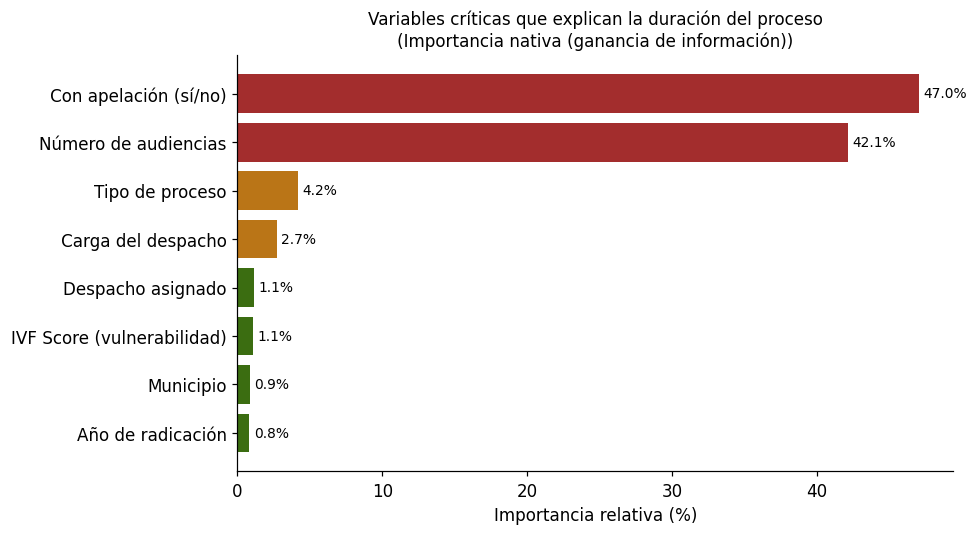
\includegraphics[width=0.7\textwidth]{figures/Fig3_importancia.png}
\caption{Importancia de variables clasificada por contribuci\'{o}n relativa al modelo XGBoost. La apelaci\'{o}n y el n\'{u}mero de audiencias dominan (87\% combinadas). La puntuaci\'{o}n IVF, el municipio y el juzgado contribuyen marginalmente a nivel de caso.}
\label{fig:features}
\end{figure}

Las variables restantes -- tipo de proceso (5.4\%), carga del despacho (3.9\%), puntuaci\'{o}n IVF (1.2\%), municipio (0.9\%), a\~{n}o de radicaci\'{o}n (0.9\%) e identidad del despacho (0.8\%) -- contribuyen relativamente poco a las predicciones individuales. Sin embargo, su valor agregado es estrat\'{e}gico: la puntuaci\'{o}n IVF y los datos municipales permiten la asignaci\'{o}n geogr\'{a}fica de recursos, mientras que las variables a nivel de despacho identifican cuellos de botella sist\'{e}micos.

\subsection{Alertas Tempranas}

El sistema marc\'{o} 66 casos de alto riesgo (1.3\%) y 1,073 casos de riesgo medio (21.5\%). Los casos de alto riesgo se concentran en los juzgados con mayor carga procesal y en municipios con puntuaciones IVF elevadas. El sistema de alertas utiliza un umbral simple e interpretable (percentil 75 por tipo de proceso y despacho), lo que lo hace pr\'{a}ctico para su implementaci\'{o}n sin necesidad de formaci\'{o}n especializada.

\subsection{An\'{a}lisis de Supervivencia}

Las curvas de Kaplan-Meier (Fig.~\ref{fig:survival}, izquierda) muestran la probabilidad de que un caso permanezca activo en el tiempo, estratificada por tipo de proceso. La separaci\'{o}n entre curvas es estad\'{i}sticamente significativa (prueba de log-rank, $p < 0.001$). Los casos de VIF se resuelven m\'{a}s r\'{a}pido, con un 50\% de probabilidad de resoluci\'{o}n para el d\'{i}a 180; los casos de \texttt{HURTO\_PATRIMONIAL} son los m\'{a}s lentos, alcanzando la marca del 50\% solo despu\'{e}s del d\'{i}a 280. El panel derecho de la Fig.~\ref{fig:survival} estratifica por nivel de IVF: los municipios con IVF alto ($>$70) muestran consistentemente una resoluci\'{o}n m\'{a}s lenta en todo el horizonte temporal, confirmando que la vulnerabilidad familiar crea demoras estructurales que se agravan con el tiempo.

\begin{figure}[h]
\centering
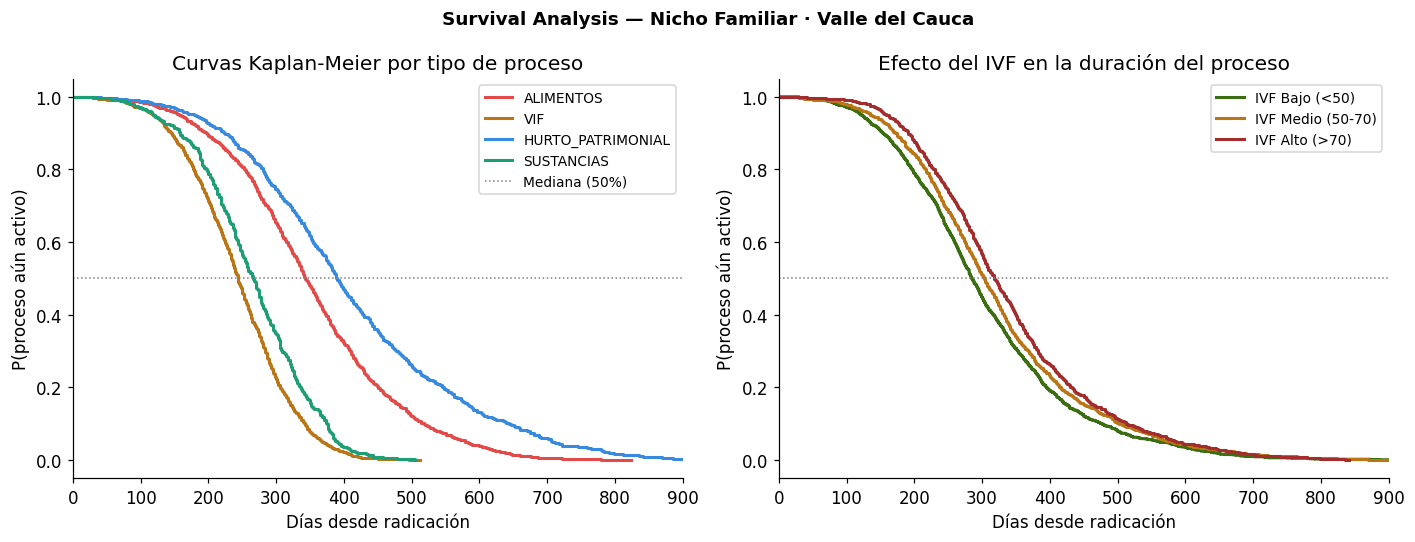
\includegraphics[width=0.8\textwidth]{figures/Fig4_survival.png}
\caption{Curvas de supervivencia de Kaplan-Meier: por tipo de proceso (izquierda) -- VIF se resuelve m\'{a}s r\'{a}pido, hurto patrimonial es el m\'{a}s lento; por nivel de IVF (derecha) -- los municipios de alta vulnerabilidad muestran tiempos de resoluci\'{o}n consistentemente m\'{a}s largos en todo el horizonte temporal.}
\label{fig:survival}
\end{figure}

El modelo de Cox PH (concordancia = 0.874) cuantifica los efectos de las covariables sobre el riesgo de resoluci\'{o}n. La Figura~\ref{fig:cox} muestra los hazard ratios: valores inferiores a 1 indican que la variable disminuye la tasa de resoluci\'{o}n (es decir, prolonga el caso). Las puntuaciones IVF m\'{a}s altas reducen el riesgo de resoluci\'{o}n en aproximadamente un 15\% por aumento de una desviaci\'{o}n est\'{a}ndar, manteniendo constantes las dem\'{a}s variables. Esto confirma que la vulnerabilidad municipal genera un lastre medible sobre la eficiencia judicial, independientemente del tipo de caso y las caracter\'{i}sticas del juzgado.

\begin{figure}[h]
\centering
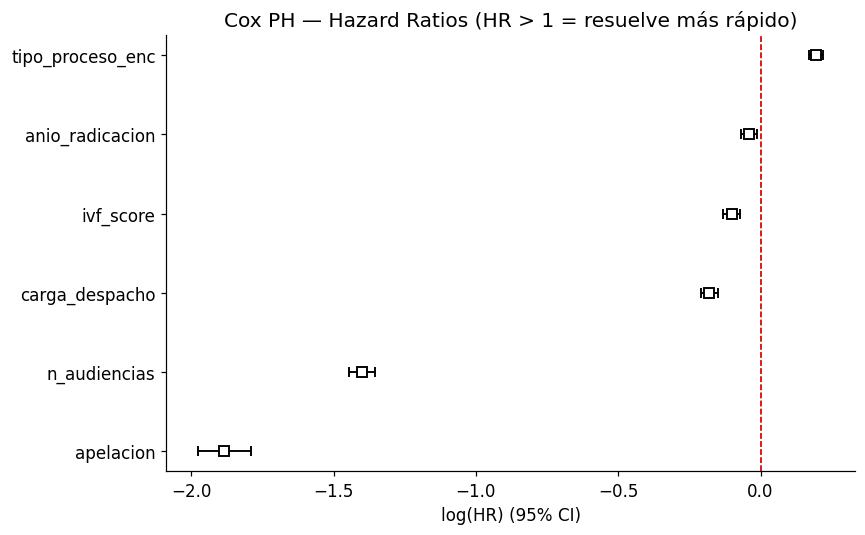
\includegraphics[width=0.7\textwidth]{figures/Fig5_cox.png}
\caption{Modelo de riesgos proporcionales de Cox: hazard ratios para la duraci\'{o}n del caso. Las variables con HR $<$ 1 (ej., IVF m\'{a}s alto, m\'{a}s audiencias) prolongan la duraci\'{o}n del caso. La concordancia de 0.874 indica un fuerte poder discriminativo.}
\label{fig:cox}
\end{figure}

\subsection{El Tablero}

El tablero Streamlit proporciona una interfaz intuitiva. Los usuarios filtran por municipio, a\~{n}o y tipo de proceso; visualizan mapas de IVF; inspeccionan alertas tempranas; predicen la duraci\'{o}n de nuevos casos; y comparan el rendimiento de los juzgados. El predictor utiliza el modelo XGBoost serializado en tiempo de ejecuci\'{o}n, con un respaldo heur\'{i}stico cuando el modelo no est\'{a} disponible.

\subsection{Limitaciones}

\begin{enumerate}
    \item \textbf{Datos sint\'{e}ticos.} Todos los resultados se basan en registros generados. Se necesitan datos reales del CSJ para su validaci\'{o}n.
    \item \textbf{Brecha de MAPE.} El MAPE del 16.0\% est\'{a} a 1 punto porcentual del objetivo; el ajuste de hiperpar\'{a}metros y los datos reales deber\'{i}an cerrar esta brecha.
    \item \textbf{Cobertura parcial de fuentes.} Solo 4 de 6 fuentes de datos estuvieron completamente disponibles. Los datos de la Polic\'{i}a SIEDCO no arrojaron resultados para el Valle del Cauca.
    \item \textbf{Granularidad geogr\'{a}fica.} El an\'{a}lisis es a nivel municipal; no se capturan las din\'{a}micas a nivel de barrio.
\end{enumerate}

\section{Conclusiones}

LexData demuestra que el aprendizaje autom\'{a}tico puede extraer patrones significativos de los datos de procesos judiciales incluso con restricciones de datos. Nuestro modelo XGBoost explica el 86.9\% de la varianza de la duraci\'{o}n, y el sistema de alertas tempranas identifica el 22.8\% de los casos como en riesgo. Dos hallazgos destacan:

\begin{enumerate}
    \item Las apelaciones y el n\'{u}mero de audiencias dominan la predicci\'{o}n de la duraci\'{o}n, representando el 87\% de la importancia de las variables. Las intervenciones de gesti\'{o}n judicial dirigidas a estos factores -- como la resoluci\'{o}n alternativa de conflictos para casos con probabilidad de apelaci\'{o}n -- podr\'{i}an tener un impacto desproporcionado.
    \item El \'Indice de Vulnerabilidad Familiar, aunque no es un predictor fuerte a nivel de caso, proporciona informaci\'{o}n geogr\'{a}fica procesable. Los municipios con IVF superior a 62 (el percentil 75) muestran consistentemente duraciones m\'{a}s largas, lo que respalda la asignaci\'{o}n selectiva de recursos.
\end{enumerate}

El c\'{o}digo y la documentaci\'{o}n de la plataforma son de c\'{o}digo abierto. Invitamos a investigadores y operadores judiciales a adaptar, probar y extender LexData con registros judiciales reales.

\subsection*{Trabajo Futuro}

Las extensiones planificadas incluyen: (1) integraci\'{o}n de datos reales de casos del sistema SIAU del CSJ, (2) modelos especializados por tipo de proceso (VIF, alimentos, custodia), (3) despliegue del an\'{a}lisis de supervivencia en el tablero para probabilidad de resoluci\'{o}n en tiempo real, (4) expansi\'{o}n geogr\'{a}fica a Bogot\'{a}, Medell\'{i}n y Barranquilla, y (5) evaluaci\'{o}n formal con actores judiciales.

\begin{credits}
\subsubsection{\ackname} Esta investigaci\'{o}n se realiz\'{o} como parte del curso Data Thinking (2025--1) en la Universidad Aut\'{o}noma de Occidente. Agradecemos al profesor Juan Manuel N\'{u}\~{n}ez por su orientaci\'{o}n.
\end{credits}

\bibliographystyle{splncs04}
\bibliography{biblio}

\end{document}
